\documentclass[hyperref={pdfpagelabels=false},t,10pt]{beamer}
\usepackage[utf8]{inputenc}
\usepackage[english]{babel}
\usepackage[T1]{fontenc}
\usepackage[default,scale=.95]{opensans}
\usepackage[most]{tcolorbox}
\usepackage{amsmath,amssymb}
\usepackage{xcolor}

%\usepackage{enumitem}



\usetheme[cd2018]{tud}
\setbeamercolor{normal text}{fg=black}
\colorlet{alert}{cdblue}
\setbeamercolor{alerted text}{fg=cdblue}
\setbeamerfont{frametitle}{size=\Large,family=\sffamily,series=\sbseries}


\DeclareRobustCommand\sbseries{\fontseries{sb}\selectfont}
\DeclareTextFontCommand{\textsb}{\sbseries}


\title{TITLE}
\author[© author]{Maik Thanh Nguyen}
\institute{Technische Universit\"at Dresden}
\datecity{CONFERENCE}
\date{DATE}

%\newtheorem{theorem}{Theorem}
%\newtheorem{definition}{Definition}
\newtheorem{claim}{Claim}
\begin{document}

%%%% Uncomment the following line to set background image to main slide
%%%% (parameter sets transparency)
%\setbeamertemplate{tud background}[image/shaded]{background.jpg}{0.5}
\addtocounter{framenumber}{-1}
\maketitle

\begin{frame}
  \frametitle{Content}

  \begin{itemize}
  \item Syntax for the basic modal language and semantics
    \begin{itemize}
        \item Kripke frames
        \item Topological space
        \item Neighbourhood frames
     \end{itemize}
  \item Multimodal logic and product of frames/spaces and logics
    \begin{itemize}
      \item Multimodal logic and product of frames
      \item Horizontal and Vertical topology/functions
      \item Product of logics and the logic T
    \end{itemize}
  \item Main result and ideas
  \end{itemize}
\end{frame}

\begin{frame}
  \frametitle{Basic modal language, Kripke frames and models}
  \begin{itemize}
    \item Basic modal langauge extends classical propositional logic. Formally:
  \end{itemize}
    
    \begin{definition}
      Let Prop be a set of variable. Then a formula $\phi$ is defined as follows:
          $$\phi ::= p \mid \bot \mid \neg \phi \mid \phi \lor \phi \mid \textcolor{red}{\Box \phi}$$
           where $\Box$ is a modal operator and $p \in$ Prop  
    \end{definition}
    %Other connectives are expressed through $\neg$ and $\lor$ and dual modal operator $\lozenge$ as $\lozenge \phi = \neg \Box \neg \phi$. 
     \pause

    \begin{definition}
    A frame $F = (W,R)$ is a pair where   
    \begin{itemize}
      \item $W$ is a non-empty set of worlds
      \item $R \subseteq W \times W $ is a binary relation
    \end{itemize}

    A model is a pair $M = (F,R)$ where $V$ is a valuation and is of the form $V : Prop \rightarrow 2^W$


    \end{definition}

\end{frame}

\begin{frame}
  \frametitle{Example}
  \begin{itemize}
    \item Let $\phi = \Box p$ and $M = (W,R,V)$ with $W = \{w_1,w_2,w_3,w_4,w_5\}$, $V(p) = \{w_3,w_4,w_5\}$ and $R = $
  \end{itemize}
  \centering
  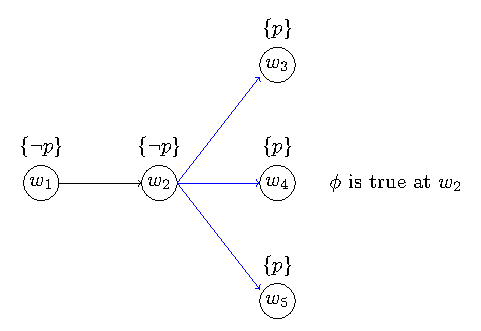
\includegraphics[width=0.55\textwidth]{Example1.pdf}
\end{frame}



\begin{frame}
  \frametitle{Kripke semantics}

  \begin{definition}
      Let $M = (F,V)$ be a model and $w \in W$ a state in $M$. A formula being true at $w$ is inductively defined as: 
      \begin{align*}
        M, w &\Vdash p &&\text{ iff } w \in V(p) \\
        M, w &\Vdash \bot  &&\text{ never } \\
        M, w &\Vdash \neg \phi &&\text{ iff not } M, w \Vdash \phi \\ 
        M, w &\Vdash \phi \lor \psi &&\text{ iff } M,w \Vdash \phi \lor M,w \Vdash \psi \\
        M, w &\Vdash \textcolor{red}{\Box \phi} &&\text{ iff } \forall v \in W : wRv \rightarrow M, v \Vdash \phi \\
        M, w &\Vdash \textcolor{red}{\lozenge \phi} &&\text{ iff } \exists v \in W : wRv \land M,v \Vdash \phi
    \end{align*}  
  \end{definition}


  
\end{frame}



\begin{frame}
  \frametitle{Topological space}
  \begin{itemize}
    \item deals with open sets, describes which points are "nearby" \pause %truth is defined differently 
    \begin{definition}
             A topological space is a pair $(X, \tau)$, where $\tau$ (called topology) is a collection of subsets of $X$ (open sets) such that: \pause
        \begin{itemize}
          \item $\emptyset$ and $X$ are open
          \item The union of arbitrary collection of open sets is open
          \item The intersection of finite collection of open sets is open
        \end{itemize} \pause
          A topological model is a structure $M = (X,\tau, \upsilon)$ where $(X, \tau)$ is a topological space and $\upsilon$ a valuation of the form $\upsilon : Prop \rightarrow 2^X$  
    \end{definition}
    \end{itemize}
    \end{frame}

  \begin{frame}
  
    \frametitle{Example}
    \begin{itemize}
      \item  Let $(X,\tau)$ be a topological space with 
      $X = \{1,2,3\}$, $\tau = \{\emptyset, \{1\}, \{2\}, \{1,2\}, W\}$ ,$V(p) = \{1,2\}$  and $\phi = \Box p$
      \pause
    \end{itemize}
    \centering
    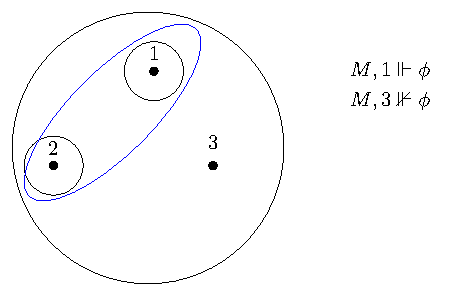
\includegraphics[width=0.55\textwidth]{Example2.pdf}

  \end{frame}


\begin{frame}
  \frametitle{Topological semantics}
  \begin{definition}
  Let $M = (X, \tau, \upsilon)$ be a topological model and $x \in X$ a point in $M$. A formula being true at $x$ is inductively defined as:

  \[
\begin{aligned}
    M, x &\vDash p &&\text{iff } x \in v(p) \\
    M, x &\vDash \bot &&\text{never} \\
    M, x &\vDash \neg \phi &&\text{iff } M, x \nvDash \phi \\
    M, x &\vDash \phi \lor \psi &&\text{iff } M, x \vDash \phi \text{ or } M, x \vDash \psi \\
    M, x &\vDash \textcolor{red}{\Box \phi} &&\text{iff }\exists U \in \tau \text{ such that } x \in U \text{ and } \forall u \in U,\; M, u \vDash \phi \\
    M, x &\vDash \textcolor{red}{\lozenge \phi} &&\text{iff }\forall U \in \tau: \text{if }x \in U \rightarrow \exists u \in U,\; M, u \vDash \phi
  \end{aligned}
\]
\end{definition}
\end{frame}




\begin{frame}
  \frametitle{Neighbourhood frames}
    \begin{itemize}
      \item Generalize Kripke semantics
      \item Captures non-normal modal logics
    \end{itemize}

    \pause
    \begin{definition}
      A neighbourhood frame is a pair $(X, \tau)$ where $\tau$ is a function $\tau : X \rightarrow 2^{2^X}$. \newline
      A neighbourhood model is a structure $M = (X, \tau, \upsilon)$, where $\upsilon$ is a valuation of the form $\upsilon : Prop \rightarrow 2^X$
    \end{definition}
\end{frame}

\begin{frame}
  \frametitle{Example}
      Assume $\phi = \Box p$. Let $W = \{1,2,3\}$, $V(p) = \{1,2\}$ and 
    \[
            \tau(x) = 
            \begin{cases}
                1 \rightarrow \{\{1\}, \{3\}, W\} \\
                2 \rightarrow \{\{2\}, \{1,2\}, W\} \\
                3 \rightarrow \{\{3\}, \{1,3\}\}
            \end{cases}
    \] 
    \centering
      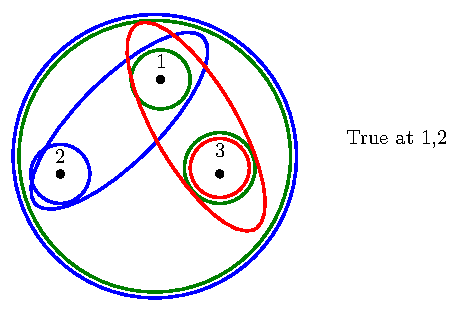
\includegraphics[width=0.55\textwidth]{Example3.pdf}
\end{frame}

\begin{frame}
  \frametitle{Neighbourhood semantics}
  \begin{definition}
  Let $M = (X,\tau,\upsilon)$ be a neighbourhood model and $x \in X$ a point in $M$. A formula being true at x is inductively defined as:
      \begin{align*}
        M,x &\Vdash p &&\text{iff } x \in V(p)\\
        M,x &\Vdash \bot &&\text{never } \\
        M,x &\Vdash \neg \phi &&\text{iff } M,x \nVdash \phi\\
        M,x &\Vdash \phi \lor \psi &&\text{iff } M,x \vDash \phi \lor M,x \vDash \psi\\
        M,x &\Vdash \textcolor{red}{\Box \phi} &&\text{iff } \exists V \in \tau(x) \forall y \in V : M,y \models \phi
    \end{align*}
  \end{definition}
\end{frame}


\begin{frame}
  \frametitle{Modal logic and the logic $T$}
  \begin{definition}
    A modal logic is a set of modal formulas containing all propositional tautologies, closed under Substitution ($\frac{\phi(p_i)}{\phi(\psi)}$), Modus Ponens $(\frac{\phi, \phi \rightarrow \psi}{\psi})$. \newline \newline \pause
    A modal logic is normal, if it contains $\Box (p \rightarrow q) \rightarrow (\Box p \rightarrow \Box q)$ (K) and is closed under Generalization $(\frac{\phi}{\Box \phi})$
  \end{definition}

  \begin{definition}
      $T = K + \Box p \rightarrow p$
  \end{definition}
\end{frame}



\begin{frame}
  \frametitle{Multimodal logic and Fusion}
  \begin{itemize}
    \item Simultaneously reasons about knowledge,time etc. 
    \item Example: combines temporal and epistemic logic to reason "when does the agent know something" \pause % consider the product of frames to interpret the formulas 
       \begin{definition}
      Let $L_1$ and $L_2$ be modal logics with one modality $\Box$. The fusion is defined as:
      $$ L_1 \otimes L_2 = K_2 + L_{1(\Box \rightarrow \Box_1)} L_{2(\Box \rightarrow \Box_2)} $$    
    \end{definition}

    %\item Let $L_1$ and $L_2$ be two modal logics with one modality $\Box$. Then the fusion
    %is defined as: $$L_1 \otimes L_2 = K_2 + L_{1 \Box \rightarrow \Box_1} + L_{2 \Box \rightarrow \Box_2}$$
   % \item we consider the product of frames to evaluate multimodal formulas
  \end{itemize}
\end{frame}

\begin{frame}
  \frametitle{Product of frames}
  \begin{itemize}
      \item Reasoning on horizontal and vertical relations in one dimension \pause% , for example we a fix time point and ask what does the agent knows at that time?
    \end{itemize}   
    \begin{definition}
      Let $F = (W, R_1)$ and $G = (V, R_2)$. We define the Kripke product on $W \times V$ as : 
        \begin{align*}
              (w,v)R_1'(w',v') &\text{ iff } wR_1w' \mbox{ and } v = v' \text{  (horizontal)} \\
              (w,v)R_2  '(w',v') &\text{ iff } w = w' \mbox{ and } vR_2v' \text{(vertical)}
      \end{align*}  

  \end{definition}
\end{frame}

\begin{frame}
  \frametitle{Example} %It’s also possible to combine modal logics with fusion
    %\centering

    \begin{tikzpicture}
       \node[draw, circle, inner sep=1.5pt] (A) at (0,0) {\small 3};
       \node[draw, circle, inner sep=1.5pt] (B) at (0,-1) {$2$};
       \node[draw, circle, inner sep=1.5pt] (C) at (0,-2) {$1$};
       \node at (-0.5,0.5) {$R_1$};

       \draw [blue,->] (C) -- (B);
       \draw [blue, ->] (B) -- (A);

       \node[draw, circle, inner sep=1.5pt] (D) at (4,-1) {$a$};
       \node[draw, circle, inner sep=1.5pt] (E) at (5,-1) {$b$};

       \draw [red, ->] (D) -- (E);
       \node at (3.5,-0.5) {$R_2$}; 
       \pause

       \node[draw, circle, inner sep=1pt] (F) at (8,0) {\small 3,a};
       \node[draw, circle, inner sep=1pt] (G) at (8,-1) {\small 2,a};
       \node[draw, circle, inner sep=1pt] (H) at (8,-2) {\small 1,a};

       \node[draw, circle, inner sep=1pt] (I) at (9,0) {\small 3,b};
       \node[draw, circle, inner sep=1pt] (J) at (9,-1) {\small 2,b};
       \node[draw, circle, inner sep=1pt] (K) at (9,-2) {\small 1,b};

       \draw [blue,->] (H) -- (G);
       \draw [blue,->] (G) -- (F);
       \draw [blue,->] (K) -- (J);
       \draw [blue,->] (J) -- (I);

       \draw [red,->] (F) -- (I);
       \draw [red,->] (G) -- (J);
       \draw [red,->] (H) -- (K);


    \end{tikzpicture}


\end{frame}

\begin{frame}
  \frametitle{Horizontal and Vertical topology}
   % \item in topological space, horizontal and vertical can be also defined \pause
  \begin{definition}
      Let \( \mathcal{X} = (X, \chi) \) and \( \mathcal{Y} = (Y, \upsilon) \) be topological spaces and \( N \subseteq X \times Y \) \newline

    \begin{description}
      \item[Horizontally open:] \(N\) is horizontally open iff 
      \[
        \forall (x, y) \in N\; \exists U \in \chi \text{ such that } x \in U \text{ and } U \times \{y\} \subseteq N.
      \]

      \item[Vertically open:] \(N\) is vertically open iff 
      \[
        \forall (x, y) \in N\; \exists V \in \upsilon \text{ such that } y \in V \text{ and } \{x\} \times V \subseteq N.
      \]

    \end{description}    
    $\tau_1$ (horizontal topology) is the set of all horizontally open sets and $\tau_2$ (vertical topology) the set of all vertically open sets.
  \end{definition}




\end{frame}

\begin{frame}
  \frametitle{Illustration, Standard product}
    \centering
    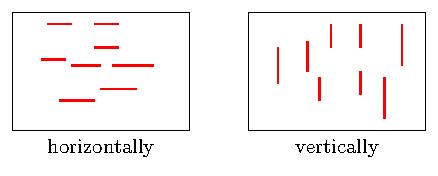
\includegraphics[width=0.55\textwidth]{Example4.pdf} \pause
  \begin{itemize}
    \item Reasoning in both directions simultaneously with the standard topology
    \item Basis of the standard topology is $\tau$ where 
    $$\tau = \{N \subseteq X \times Y \mid \exists U \in \chi \exists V \in \upsilon: N = U \times V\}$$  
  \end{itemize}

\end{frame}

\begin{frame}
  \frametitle{Horizontal, Vertical and Standard functions}
  \begin{definition}
    Let $\mathcal{X}$ = ($X$, $\tau_1$) and $\mathcal{Y}$ = ($Y$, $\tau_2$) be two n-frames. We define the full product as
      $$\mathcal{X} \times_n^+  \mathcal{Y} = (X \times Y, \tau_1', \tau_2', \tau) \text{ where}$$
      $$ \tau_1'(x,y) = \{ U \subseteq \mbox{X} \times \mbox{Y} \mid \exists V \in \tau_1(x) : V \times  \{ y \} \subseteq U \}$$
      $$ \tau_2'(x,y) = \{ U \subseteq \mbox{X} \times \mbox{Y} \mid \exists V \in \tau_2(y) : \{ x \} \times V \subseteq U \}$$
          $$ \tau(x,y) = \{ U \subseteq \mbox{X} \times \mbox{Y} \mid \exists W \in \tau_1(x) \, \exists V \in \tau_2(y) : W \times V \subseteq U \}$$      
  \end{definition}

\end{frame}

\begin{frame}
  \frametitle{Product of logics }
  \begin{definition}
    Let $L_1$ and $L_2$ be two unimodal logic. We define the full n-product of them as:
    $$L_1 \times_n^+ L_2 =  Log(\{\mathcal{X} \times_n^+ \mathcal{Y} \mid \mathcal{X} \Vdash L_1 \text{ and } \mathcal{Y} \Vdash L_2 \})$$   
    where $Log(\mathcal{C}) = \{\phi \mid F \Vdash \phi \text{ for } F \in \mathcal{C}\}$
  \end{definition}


\end{frame}

\begin{frame}
  \frametitle{Main Research Question}
    \begin{theorem}
      $$T \otimes T \otimes T + \Box p \rightarrow \Box_1 p \land \Box_2 p = T \times_n^+ T$$
          \end{theorem}\pause


  \begin{itemize}
    \item $T \otimes T \otimes T = K_3 + T_{\Box} + T_{(\Box \rightarrow \Box_1)} + T_{(\Box \rightarrow \Box_2)}$ is the logic with three modalities 
    \item $\Box p \rightarrow \Box_1 p \land \Box_2 p$ is the interaction axiom \pause
    \item Sketch the inclusion from right to left
    \item Proof is splitted into two parts (ideas are from [1], [2])
  \end{itemize}
\end{frame}

\begin{frame}
  \frametitle{Sketch of the main ideas}
  \begin{itemize}
    \item Pick $\mathcal{C} = \{F \mid F \Vdash T \otimes T\otimes T + \Box p \rightarrow \Box_1 p \land \Box_2 p\}$  \pause
    \end{itemize}

    \begin{claim}
      $Log(\mathcal{C}) = T \otimes T \otimes T + \Box p \rightarrow \Box_1 p \land \Box_2 p$
    \end{claim} \pause

    \begin{itemize}
      \item  Shown by \textcolor{red}{Sahlqvist Theorem}
    \end{itemize}
    \pause

    \begin{claim}
      $T \otimes T \otimes T + \Box p \rightarrow \Box_1 p \land \Box_2 p$ has the finite model property
    \end{claim}
    \pause

    \begin{itemize}
      \item Use \textcolor{red}{Filtration Theorem}
    \end{itemize}

    %\item Show $Log(T_{\omega,\omega,\omega[rn]}) = T \otimes T \otimes T+ \Box p \rightarrow \Box_1 p \land \Box_2 p$
   % \item By FMP pick a finite frame $F \in \mathcal{C}$ and construct a bounded morphism from $T_{\omega,\omega,\omega[rn]}$ to $F$


\end{frame}

\begin{frame}
  \frametitle{Sketch continue}
  \begin{itemize}
    \item Construct an infinite branching and infinite depth tree with three reflexive relations ($T_{\omega,\omega,\omega[rn]}$) \pause
  \end{itemize}
  \centering
  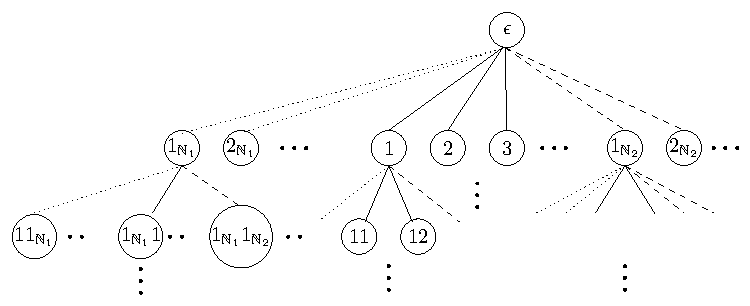
\includegraphics[width=0.73\textwidth]{Example7.pdf}
    
  \end{frame}

  \begin{frame}
    \frametitle{Sketch continue}
    \begin{definition}
      Let $F = (W,R_1,R_2,...)$ and $F' = (W',R_1',R_2',...)$ be two frames. A bounded morphism $f: W \rightarrow W'$ can be illustrated as:  
      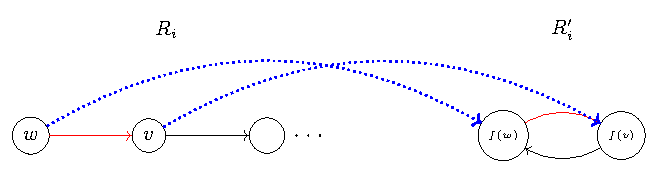
\includegraphics[width=0.73\textwidth]{Example8.pdf}
    
    \vspace{0.5cm}
    \begin{tikzpicture}
      \node[draw, circle, minimum size=0.2cm] (A) at (0,0) {$w$};
      \node[draw, circle, minimum size=0.2cm] (B) at (0,-1.5) {$v$};
      \node[draw, circle, font=\tiny\itshape] (C) at (1.8,0) {$f(w)$};
      \node[draw, circle, font=\tiny\itshape] (D) at (1.8,-1.5){$f(v)$};
      

      \draw [->] (C) -- (D);
      \draw[->, bend left=30,dotted, thick] (A) to (C); \pause
      \draw [->,red] (A) -- (B);
      \draw [->, bend left=330,dotted, thick,red] (B) to (D);
    \end{tikzpicture}
    \end{definition} 

  \end{frame}

  \begin{frame}
    \frametitle{Sketch continue}
    \begin{claim}
       $Log(T_{\omega,\omega,\omega[rn]}) = T \otimes T \otimes T+ \Box p \rightarrow \Box_1 p \land \Box_2 p$   
    \end{claim}
    
  \end{frame} 

\begin{frame}
  \frametitle{Detailed sketch}
  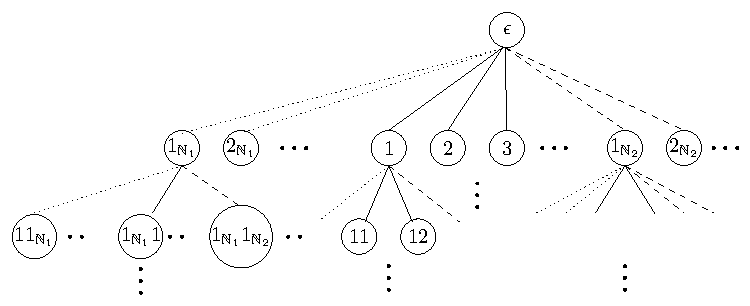
\includegraphics[width=0.73\textwidth]{Example7.pdf} \newline\pause

  \begin{tikzpicture}[yshift=-0.15cm]
    \node[draw, circle, minimum size=0.2cm] (A) at (0,0) {$x$};
    \node[draw, circle, minimum size=0.2cm] (B) at (1,1) {$y$};
    \node[draw, circle, minimum size=0.2cm] (C) at (1,-1) {$z$};
    \draw [->] (A) to (B);
    \draw [->] (A) to (C);

    \node at (-0.5,1.5) {$R_1'$};

    \node[draw, circle, minimum size=0.2cm] (D) at (4,0) {$x$};
    \node[draw, circle, minimum size=0.2cm] (E) at (5,1) {$y$};
    \node[draw, circle, minimum size=0.2cm] (F) at (5,-1) {$z$};
    \draw [->] (D) to (E);
    \draw [->] (E) to (F);

    \node at (3.5,1.5) {$R_2'$};

    \node[draw, circle, minimum size=0.2cm] (G) at (7.5,0) {$x$};
    \node[draw, circle, minimum size=0.2cm] (H) at (9,1) {$y$};
    \node[draw, circle, minimum size=0.2cm] (I) at (9,-1) {$z$};

    \draw [->] (G) to (H);
    \draw [->] (G) to (I);

    \draw[->,  bend left=30, thick] (H) to (I);
    \draw[->, bend left=30,thick] (I) to (H);

    \node at (7.5,1.5) {$R'$};
    \pause



  \end{tikzpicture}
\end{frame}


\begin{frame}
  \frametitle{Required components}
  $$Log(T_{\omega,\omega,\omega[rn]}) = T \otimes T \otimes T+ \Box p \rightarrow \Box_1 p \land \Box_2 p$$
  \begin{itemize}
    \item Introduce $T_{\omega[rn]}$ a simpler version of $T_{\omega,\omega,\omega[rn]}$  \pause
    \item Construct  $N_\omega(T_{\omega[rn]})$ the neighbourhood version of $T_{\omega[rn]}$
    \item Show $T = Log(N_\omega(T_{\omega[rn]}))$ \pause
    \item Construct a bounded morphism $$N_\omega(T_{\omega[rn]}) \times_n^+ N_\omega(T_{\omega[rn]}) \rightarrow T_{\omega,\omega,\omega[rn]}$$
    \item With some further steps we can conclude $$T \times_n^+ T \subseteq T \otimes T \otimes T + \Box p \rightarrow \Box_1 p \land \Box_2 p$$
  \end{itemize}

\end{frame} 


\begin{frame}
  \frametitle{Future works}
  \begin{itemize}
    \item Many ways to continue the research
    \item Discover how it works for logic $K$
    \item Combine different logics for example $D \times_n^+ K, T \times_n^+ K, ...$
    \item For logic $\Lambda$ with $T \subseteq \Lambda \subseteq S4$, does the following hold:
     $$\Lambda \otimes \Lambda \otimes \Lambda + \Box p \rightarrow \Box_1 p \land \Box_2 p = \Lambda \times_n^+ \Lambda$$
  
  \end{itemize}
\end{frame}

\begin{frame}
  \vspace{3.5cm}
  \centering
  \begin{tikzpicture}
    \node[font=\Large] at (0,0) {Conclusion};
  \end{tikzpicture}
\end{frame}

\begin{frame}
  \frametitle{References}
    [1] Johan van Benthem, Guram Bezhanishvili, Balder ten Cate, and Darko Sarenac.\\
    Multimodal logics of products of topologies. \textit{Studia Logica}, 84:369–392, 2006. \newline

    [2] Andrei Kudinov. Modal logic of some products of neighbourhood frames.\\
    In \textit{Advances in Modal Logic, Volume 9}, pages 286–294, London, 2012. College Publications.
\end{frame}


\end{document}
